\subsection{Extended Kalman Filter}
The Kalman filter provides optimal state estimation for linear systems under Gaussian noise assumptions. However, most real world systems such as those involving vehicle dynamics, navigation, or orientation estimation are inherently nonlinear. To handle such systems, the Extended Kalman Filter (EKF) generalizes the Kalman filter framework by linearizing the nonlinear system around the current state estimate. This allows the Kalman filter formulation to be applied locally in a linearized form, maintaining recursive estimation in nonlinear environments.  
\\ \\
The nonlinear system and measurement models are expressed as
$$
    \mathbf{x}_{k+1} = f(\mathbf{x}_k, \mathbf{u}_k) + \mathbf{w}_k, \qquad
    \mathbf{z}_k = h(\mathbf{x}_k) + \mathbf{v}_k
$$
where $\mathbf{x}_k$ is the system state, $\mathbf{u}_k$ is the control input, and $\mathbf{z}_k$ is the measurement vector. The process and measurement noises $\mathbf{w}_k$ and $\mathbf{v}_k$ are assumed to be zero mean, white, and Gaussian distributed with covariances $Q$ and $R$, respectively.  
\\ \\
To apply the Kalman filter framework, the nonlinear functions $f(\cdot)$ and $h(\cdot)$ must be approximated by their first order Taylor expansion around the current state estimate $\hat{\mathbf{x}}_{k|k-1}$. This yields the linearized system matrices
$$
    F_k = \left.\frac{\partial f}{\partial \mathbf{x}}\right|_{\hat{\mathbf{x}}_{k|k-1}, \mathbf{u}_k}, \qquad
    H_k = \left.\frac{\partial h}{\partial \mathbf{x}}\right|_{\hat{\mathbf{x}}_{k|k-1}}
$$
The Jacobian matrices $F_k$ and $H_k$ describe how small perturbations in the state affect the predicted dynamics and the expected measurements. This linearization step is local and valid only within the vicinity of the current state estimate, as illustrated in Figure \ref{fig:state-estimation-extended-kalman-filter}.  
\\ \\
\begin{figure}[H]
    \centering
    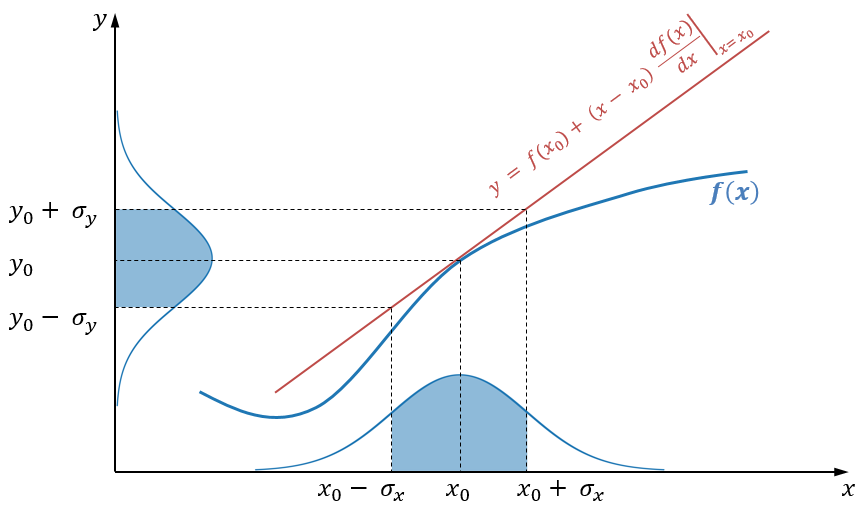
\includegraphics[width=1.0\linewidth]{Pictures/State_Estimation/Extended_Kalman_Filter/Extended_Kalman_Filter_Illustrated.png}
    \caption{Illustration of local linearization in the Extended Kalman Filter. The nonlinear function $f(x)$ is approximated by its tangent around the current estimate, allowing local linear propagation. Image taken from Alex Becker's \textit{``Introduction to Kalman Filtering''}.\textsuperscript{\cite{extended_kalman_filter}}}
    \label{fig:state-estimation-extended-kalman-filter}
\end{figure}
\noindent
An accurate discretization of the continuous time dynamics is essential to ensure consistent state propagation. In this work, the continuous model $\dot{\mathbf{x}} = A\mathbf{x} + B\mathbf{u}$ is discretized using the \textit{``Zero-Order Hold (ZOH)''} method, which assumes that the control input remains constant within each sampling interval $[k\Delta t, (k+1)\Delta t)$.  
\\ \\
The resulting discrete time model is given by
$$
    \mathbf{x}_{k+1} = F_k\mathbf{x}_k + G_k\mathbf{u}_k,
$$
where
$$
    F_k = e^{A\Delta t}, \qquad
    G_k = \int_0^{\Delta t} e^{A\tau}B\,d\tau.
$$
This can be computed compactly using the augmented matrix exponential
$$
    e\,^{
        \begin{bmatrix}
            A & B \\ 
            0 & 0
        \end{bmatrix}
        \Delta t
        }
    =
    \begin{bmatrix}
        F_k & G_k \\
        0 & I
    \end{bmatrix}.
$$
The ZOH method preserves both the stability and dynamic behavior of the original continuous time system exactly for LTI models. It provides a numerically stable and accurate discretization, making it particularly suitable for embedded real-time implementations.  
\\ \\
In digital systems, the matrix exponential $e^{A\Delta t}$ cannot be computed analytically and must be approximated numerically. A reliable and efficient method is the \textit{``Padé approximation with scaling and squaring''}, which provides a good balance between computational speed and numerical accuracy.  
\\ \\
The Padé approximation expresses the exponential as a rational function:
$$
    e^{A} \approx \left(I - \frac{A}{2} + \frac{A^2}{12} - \frac{A^3}{120} + \dots \right)^{-1}
                  \left(I + \frac{A}{2} + \frac{A^2}{12} + \frac{A^3}{120} + \dots \right),
$$
where higher order terms improve accuracy at the cost of computation. To avoid instability for large $\|A\|$, the matrix is first scaled down by a power of two, computed as
$$
    A_s = \frac{A}{2^s},
$$
where $s$ is chosen such that $\|A_s\|$ is below a defined threshold. The exponential of $A_s$ is then computed using the Padé rational form, and the final result is obtained by repeated squaring:
$$
    e^A = (e^{A_s})^{2^s}.
$$
This method ensures stable and efficient computation of matrix exponentials even for high order systems, making it practical for embedded discretization of continuous time models.  
\\ \\
When using nonlinear dynamics, the continuous time system is generally expressed as
$$
    \dot{\mathbf{x}} = f(\mathbf{x}, \mathbf{u}).
$$
To implement the continuous time dynamics $\dot{\mathbf{x}} = f(\mathbf{x}, \mathbf{u})$ on a digital system, the time derivative must be approximated numerically. This is achieved through time discretization, where the continuous evolution of the state is expressed as a difference equation over discrete sampling intervals.  
\\ \\
One of the simplest and most widely used discretization schemes is the forward (Newton-Euler) method.
$$
    \mathbf{x}_{k+1} \approx \mathbf{x}_k + \Delta t \, f(\mathbf{x}_k, \mathbf{u}_k).
$$  
\\ \\
In this discrete form, the function $f(\mathbf{x}, \mathbf{u})$ used within the EKF no longer represents the instantaneous derivative $\dot{\mathbf{x}}$, but rather the integrated or \textit{``propagated''} state over one time step. For notational simplicity, many EKF formulations redefine the discrete transition function as
$$
    f_d(\mathbf{x}_k, \mathbf{u}_k) = \mathbf{x}_k + \Delta t \, f(\mathbf{x}_k, \mathbf{u}_k),
$$
where $f_d(\cdot)$ implicitly includes the time step integration. This convention is used throughout this work to maintain concise notation while ensuring consistency with the underlying continuous time model.
\\ \\
The EKF prediction and update steps then follow directly from the linearized system. During the \textit{``prediction step''}, the nonlinear process model is propagated as
$$
    \hat{\mathbf{x}}_{k|k-1} = f_d(\hat{\mathbf{x}}_{k-1|k-1}, \mathbf{u}_{k-1}),
$$
and the covariance prediction is computed using the linearized Jacobian:
$$
    P_{k|k-1} = F_k P_{k-1|k-1} F_k^\top + Q.
$$
The \textit{``update step''} corrects the predicted estimate using the measurement model:
$$
\begin{aligned}
    K_k &= P_{k|k-1}H_k^\top(H_kP_{k|k-1}H_k^\top + R)^{-1}, \\
    \hat{\mathbf{x}}_{k|k} &= \hat{\mathbf{x}}_{k|k-1} + K_k[\mathbf{z}_k - h(\hat{\mathbf{x}}_{k|k-1})], \\
    P_{k|k} &= (I - K_kH_k)P_{k|k-1}.
\end{aligned}
$$
After each update, attitude states represented by quaternions are normalized to maintain a valid unit quaternion. This step is crucial in inertial navigation systems, as numerical drift in the quaternion magnitude can lead to significant orientation errors over time. The normalization ensures that the quaternion remains on the unit hypersphere, preserving a valid rotation representation:
$$
    \mathbf{q}_{k|k} \leftarrow \frac{\mathbf{q}_{k|k}}{\|\mathbf{q}_{k|k}\|}.
$$
Here, $\mathbf{q}_{k|k}$ denotes the updated quaternion after the correction step, and $\|\mathbf{q}_{k|k}\|$ is its Euclidean norm. This operation enforces the constraint $\|\mathbf{q}\| = 1$, guaranteeing that the quaternion continues to represent a proper rotation without scale distortion.
\\ \\
The EKF provides a computationally efficient framework for nonlinear estimation. However, it relies heavily on the validity of local linearization, which may lead to divergence if the system dynamics are strongly nonlinear or the initial state uncertainty is large. In particular, when dealing with orientation states represented by quaternions or with highly coupled nonlinear motion models such as those in INS, the EKFs 1st order approximation may fail to capture the true system behavior.  
\\ \\
Despite these limitations, the EKF remains widely used in embedded navigation systems due to its simplicity, real-time efficiency, and well understood theoretical foundation. An important improvement to the EKF is the Error State Kalman Filter (ESKF), which reformulates the estimation problem by linearizing not around the full nominal states but around the small error states instead. These error variables tend to behave more linearly and remain bounded, resulting in improved numerical stability and consistency, especially for systems with rotational dynamics such as those using quaternions. Essentially, the ESKF provides a smarter way to linearize highly nonlinear systems by focusing on the deviation from the nominal trajectory rather than the absolute state itself. For applications requiring even higher robustness to nonlinearity, alternative methods such as the Unscented Kalman Filter (UKF) or manifold based approaches can provide improved performance at the cost of increased computational complexity.

